\section{Dependency Management \& Plugin}
Una delle parti più importanti di uno strumento di questo tipo è la gestione delle dipendenze che si divide in 2 parti: incoming files e outgoing files. Gradle ha bisogno di conoscere di cosa il nostro progetto ha bisogno per poter essere compilato ed eseguito le così dette dipendenze (dipendencies) che in questo caso sono gli incoming files. Gli outgoing files sono invece tutto ciò che il progetto produce, definite pubblicazioni (pubblications). Le dipendenze vengono specificate in forma di modules, è quindi necessario indicare dove si trovano questi modules in modo tale che Gradle li possa scaricare e impostare per il progetto che stiamo sviluppando. La posizione dove è possibile trovare i modules è definita repository, è necessario quindi dichiarare le repositories usate per le dipendenze volute. Ci sono 2 tipi di repository: 
\begin{enumerate}
    \item esterne, in questo caso la repository si trova in un server online adibito alla raccolta di modules
    \item interne, la repository è una cartella locale al progetto
\end{enumerate}
Per quanto riguarda quelle esterne Gradle si occuperà di scaricarle. E' possibile che alcune dipendenze vengano usate in più progetti, gradle mantiene quindi una cache locale, chiamata dependency cache, in cui salverà i modules già scaricati in modo da evitare di effettuare il download ad ogni build. Possiamo quindi immaginare che il ciclo di risoluzione delle dipendenze esterne sarà questo:
\begin{enumerate}
    \item ricerca delle dipendenze esterne nella cache locale
    \item se non si trovano nella cache locale si controlla se esistono nelle repository specificate
    \item se sono state trovate, vengono scaricate e inserite nella cache locale
\end{enumerate}
Nell'immagine è possibile vedere il percorso specifico che effettua la dependency resolution di Gradle:
\begin{figure}[H]
\centering
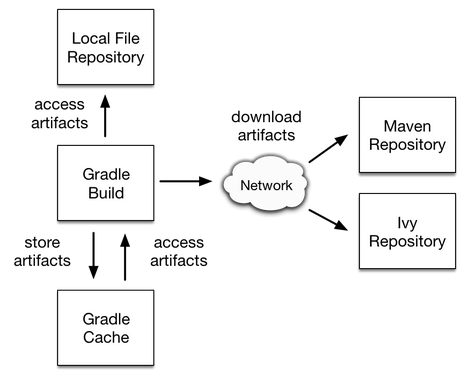
\includegraphics[width=0.4\linewidth]{3DependencyManagement/depMan.png}
\end{figure}
Analizziamo ora il caso di un progetto java.

\subsection{Java Plugin}
Prima di tutto è necessario indicare in che linguaggio il nostro progetto viene rilasciato (consideriamo d'ora in poi solo il caso di Java), possiamo farlo in 2 modi:
\begin{enumerate}
    \item aggiungere al file build.gradle:
    \begin{lstlisting}[frame=single]
apply plugin: 'java' \end{lstlisting}
    \item aggiungere al file build.gradle:
    \begin{lstlisting}[frame=single]
plugins {
    id 'java'
}
    \end{lstlisting}
\end{enumerate}
Questo aggiungerà vari tasks necessari ad un progetto in java:
\begin{figure}[H]
    \centering
    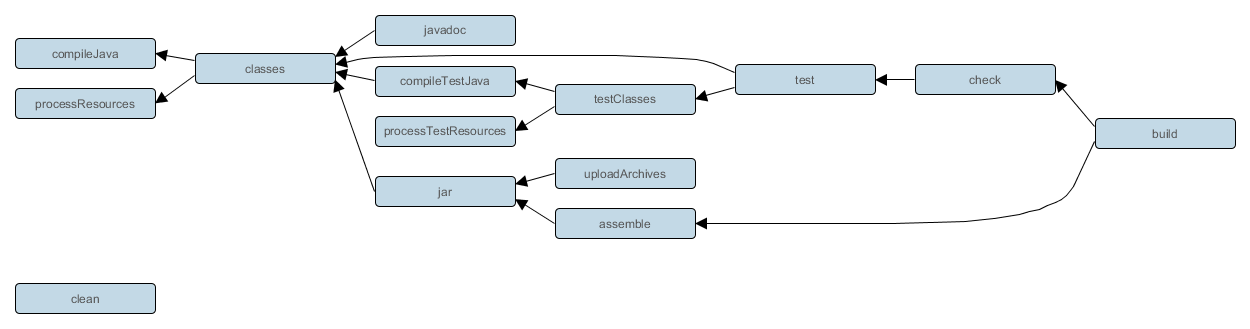
\includegraphics[width=1.0\linewidth]{3DependencyManagement/javaPlug/javaPluginTasks.png}
    \label{fig:my_label}
\end{figure}
A questo punto per poter usufruire di una dipendenza è necessario specificare da dove Gradle deve andare a prenderla, dobbiamo quindi indicare il repository remoto di riferimento. Se per esempio vogliamo che il nostro repository di riferimento sia Maven allora dobbiamo aggiungere al build.gradle:
\begin{lstlisting}[frame=single]
repositories {
    mavenCentral()
} \end{lstlisting}
In questo modo tutte le dipendenze che andremo a indicare successivamente saranno riferimenti alle pubblicazioni su Maven Central. La dichiarazione delle dipendenze deve essere inserita nel tag \texttt{dependencies} nel build.gradle file. Per esempio vogliamo avere junit 4.12 come dipendenza al nostro progetto Gradle allora dobbiamo aggiungere:
\begin{lstlisting}[frame=single]
dependencies {
    testImplementation group: 'junit', name: 'junit', version: '4.12' 
} \end{lstlisting}
Osserviamo che nella dichiarazione ci sono 4 diversi indicatori:
\begin{itemize}
    \item \texttt{testImplementation} indica la configurazione della dipendenza, in questo caso sarà importata durante l'implementazione dei test;
    \item \texttt{group, name, version} corrispondono rispettivamente al groupId (nome del team o della società che ha sviluppato il modulo), artifactId (nome effettivo del modulo) e al version (versione del modulo) definiti su Maven.
\end{itemize}
Esiste un modo molto più diretto per indicare una dipendenza:
\begin{lstlisting}[frame=single]
dependencies {
    testImplementation 'junit:junit:4.12'
} \end{lstlisting}
Ha lo stesso significato precedente ma ha una forma più compatta, forma che adotta anche la documentazione Maven:
\begin{figure}[H]
\centering
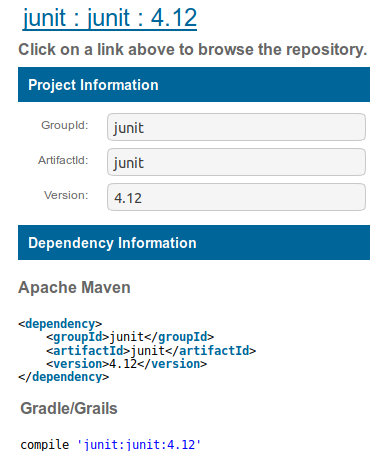
\includegraphics[width=0.4\linewidth]{3DependencyManagement/javaPlug/gradleInMavenRepo.png}
\end{figure}
Spesso in un progetto non è necessario specificare il numero dell'aggiornamento della versione, ma basta la versione più aggiornata, questo è possibile indicarlo a gradle con un \texttt{+} subito dopo la versione voluta:
\begin{lstlisting}[frame=single]
dependencies {
    testImplementation 'junit:junit:4.+'
} \end{lstlisting}
In questo modo quando eseguiremo il task \texttt{dependencies} gradle si assicurerà che la versione in uso di quella dipendenza specifica sia l'ultima rilasciata. Possiamo notare ora la differenza sostanziale della configurazione delle dipendenze tra il pom.xml di Maven e il build.gradle di Gradle. A questo punto per scaricare le dipendenze si deve eseguire il comando \texttt{dependencies} il cui output restituirà una lista di tutte le configurazioni con le relative dipendenze associate (non mostro tutto l'output perchè è molto corposo):
\begin{verbatim}
> Task :dependencies 

------------------------------------------------------------
Root project
------------------------------------------------------------

[...]

compile - Dependencies for source set 'main' (deprecated, use 'implementation ' instead).
No dependencies

[...]

default - Configuration for default artifacts.
No dependencies

[...]

runtime - Runtime dependencies for source set 'main' (deprecated, use 'runtimeOnly ' instead).
No dependencies

[...]

testCompileClasspath - Compile classpath for source set 'test'.
\--- junit:junit:4.+ -> 4.12
     \--- org.hamcrest:hamcrest-core:1.3

testCompileOnly - Compile only dependencies for source set 'test'.
No dependencies

testImplementation - Implementation only dependencies for source set 'test'. (n)
\--- junit:junit:4.+ (n)

testRuntime - Runtime dependencies for source set 'test' (deprecated, use 'testRuntimeOnly ' instead).
No dependencies

testRuntimeClasspath - Runtime classpath of source set 'test'.
\--- junit:junit:4.+ -> 4.12
     \--- org.hamcrest:hamcrest-core:1.3

[...]

BUILD SUCCESSFUL in 0s
1 actionable task: 1 executed \end{verbatim}
Come è possibile notare dall'output esistono molte configurazioni associabili a una dipendenza: compile, default, runtime, testImplementation, e così via, ognuno dei ha uno scopo ben preciso. Possiamo dividere le configurazioni in 3 scopi principali:
\begin{enumerate}
    \item \texttt{implementation}, sono le dipendenze necessarie per compilare il source del progetto che non devono comparire nell'API
    \item \texttt{api}, sono le dipendenze necessarie per compilare il source del progetto che devono comparire nell'API
    \item \texttt{testImplementation}, sono le dipendenze necessarie per compilare ed eseguire i test associati alla source del progetto
\end{enumerate}
I tasks aggiunti da questo plugin assume che il layout del progetto sia di questo tipo:
\begin{center}
\begin{tabular}{|c|c|}
\hline
Directory & Meaning  \\
\hline
\hline
    src/main/java & Sorgente del codice Java\\
    src/main/resources & Risorse \\
    src/test/java & Sorgente del codice di Test \\
    src/test/resources & Risorse usate dai test \\
\hline
\end{tabular}
\end{center}
Tutto questo è automatizzato dal comando:
\begin{verbatim}
    $ gradle init --type java-application\end{verbatim}
Che creerà lo scheletro di un progetto standard Java per sviluppare un applicativo (nel caso si voglia sviluppare una libraria si deve usare il tipo \texttt{java-library}). Il task sicuramente più usato in un progetto è \texttt{test}, questo task è una istanza della classe \texttt{Test} definita da Gradle (consultabile nell'API: \textit{\href{https://docs.gradle.org/current/dsl/org.gradle.api.tasks.testing.Test.html}{docs.gradle.org/current/dsl/org.gradle.api.tasks.testing.Test.html}}) che individua automaticamente tutti gli unit test all'interno della cartella in cui si trova il codice di test, di default nella directory: \texttt{src/test/java}, e li esegue. Può far molto comodo sapere che esiste un opzione \texttt{--continuous} che consente di eseguire un task tutte le volte che viene modificato un file del progetto:
\begin{verbatim}
    $ gradle test --continuous\end{verbatim}
Questo permetterà di controllare ad ogni modifica se la build fallirà o avrà successo. Inolte la build di questo task eseguirà tutti i test dal primo all'ultimo anche se uno di questi fallisce, per progetti di grosse dimensioni quindi questo potrebbe essere uno spreco di risorse. Per indicare alla build di fallire appena un test fallisce ci sono diversi modi:
\begin{enumerate}
    \item Settare la proprietà \texttt{failFast} a true per il task \texttt{test} direttamente nel file di configurazione gradle:
    \begin{lstlisting}[frame=single]
    test {
        failFast = true
    }
    \end{lstlisting}
    \item Indicarlo direttamente da linea di comando, usando l'opzione \texttt{--fail-fast}, nel nostro caso:
\begin{verbatim}
    $ gradle test --fail-fast \end{verbatim}
\end{enumerate}
Questo permetterà di diminuire i tempi di attesa non necessari, facendo fallire al primo test non giusto. Un'altra importante funzionalità di Gradle per quanto riguarda i test è quello di poter specificare dei filtri che indicano con precisione quali test eseguire, per esempio se volessimo eseguire una sola classe di test. Per fare questo ci sono 2 modi:
\begin{enumerate}
    \item Impostare il filtro direttamente nel file di configurazione gradle:
    \begin{lstlisting}[frame=single]
    test {
        filter {
            includeTestsMatching <package>
            includeTestsMatching <methodName>
        }
    }
    \end{lstlisting}
    I filtri supportano anche l'uso delle wildcards "*", per esempio se volessimo eseguire solo gli integration tests e i test del package org.example.app dovremo definire 2 filtri:
    \begin{lstlisting}[frame=single]
    test {
        filter {
            includeTestsMatching "org.example.app.*"
            includeTestsMatching "*IntegTest"
        }
    }
    \end{lstlisting}
    \item Indicare direttamente da linea di comanda per un unica build, usando l'opzione \texttt{--tests}:
    \begin{verbatim}
    $ gradle test --tests <filtro> \end{verbatim}
    Per esempio se volessimo eseguire il metodo di test someFeature della classe SomeTest che si trova nel package org.example.app allora dovremmo eseguire:
    \begin{verbatim}
    $ gradle test --tests org.example.app.SomeTest.someFeature \end{verbatim}
    Oppure volessimo eseguire tutti gli integration tests:
    \begin{verbatim}
    $ gradle test --tests \*IntegTest \end{verbatim}
\end{enumerate}
Ovviamente il secondo caso è quello comunemente usato per eseguire build specifici su una singola classe, evitando di modificare i filtri nel build.gradle. Un altro task importante per il rilascio di un applicativo è \texttt{jar} che crea un file JAR contenente: classi, files e risorse usate. Per essere eseguito questo task necessita la definizione di alcune proprietà:
\begin{itemize}
    \item Titolo del progetto 
    \item Versione del progetto 
    \item Classe in cui si trova il main del progetto (questo viene definito solo nel caso in cui si debba rilasciare un eseguibile) 
\end{itemize}
Queste devono essere inserite nel così detto \textbf{MANIFEST}, andiamo quindi a definire il campo manifest per il task jar:
\begin{lstlisting} [frame=single]
jar {
    manifest {
        attributes("Implementation-Title": "Example",  "Implementation-Version": 1.0, 'Main-Class': 'app')
    }    
}
\end{lstlisting}

\subsection{Eclipse plugin}
Gradle mette a disposizione anche dei plugin esclusivi per gli IDE (Integrated development environment). Considereremo il caso dell'IDE Eclipse a cui sono associati 2 plugin:
\begin{itemize}
    \item \texttt{eclipse-wtp} (Eclipse Web Tools Platform Project)
    \item \texttt{eclipse}
\end{itemize}
Questi plugin aggiungono alcuni tasks molto importanti per progetti sviluppati su questo IDE (è possibile trovare tutti i task nella documentazione relativa: \textit{\href{https://docs.gradle.org/current/userguide/eclipse\_plugin.html\#sec:eclipse\_tasks}{docs.gradle.org/current/userguide/eclipse\_plugin.html}}). Creiamo quindi un nuovo progetto java eseguendo il task init:
\begin{verbatim}
    $ gradle init --type java-application\end{verbatim}
Andiamo a modificare il build.gradle aggiungendo il plugin \texttt{eclipse}:
 \begin{lstlisting}[frame=single]
plugins {
    id 'eclipse'
} \end{lstlisting}
Se andiamo ora a eseguire la build tasks per vedere quali tasks il nostro progetto Gradle ha a disposizione vedremo che nell'output ci sarà una sezione definita \textbf{IDE tasks}:
\begin{verbatim}
IDE tasks
---------
cleanEclipse - Cleans all Eclipse files.
eclipse - Generates all Eclipse files. \end{verbatim}
Possiamo ora quindi eseguire la build \texttt{eclipse} per generare tutti i file necessari per un progetto eclipse:
\begin{verbatim}
    $ ./gradlew eclipse\end{verbatim}
La build genererà 2 files che sono: \texttt{.classpath} e \texttt{.project}, e 1 directory che è \texttt{.settings}, questi 3 elementi servono all'IDE per identificare e generare i dati di un progetto. A questo punto possiamo aprire eclipse e importare il progetto che abbiamo appena creato:
\begin{figure}[H]
    \centering
    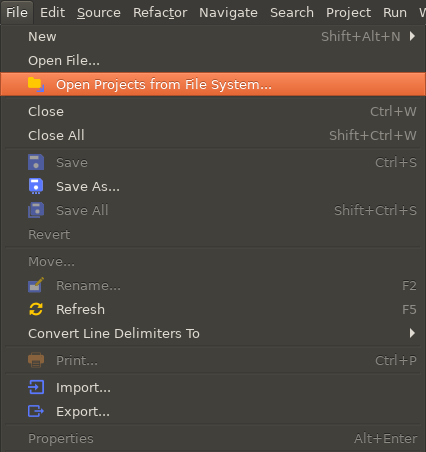
\includegraphics[width=0.4\linewidth]{3DependencyManagement/eclipsePlugin/openProject.png}
\end{figure}
Si aprirà una finestra in cui ci sarà un campo \texttt{import source} dove dovremo indicare il percorso specifico del progetto. Il risultato sarà un progetto contenente questo:
\begin{figure}[H]
    \centering
    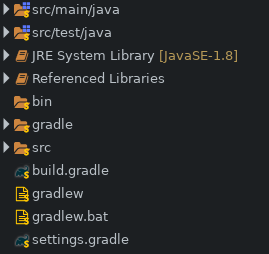
\includegraphics[width=0.4\linewidth]{3DependencyManagement/eclipsePlugin/resultProject.png}
\end{figure}
Tutto questo procedimento è possibile farlo direttamente da Eclipse, infatti installando il plugin chiamato \texttt{Buildship Gradle Integration 2.0} è possibile creare un nuovo progetto Gradle. Per farlo basterà cliccare su \texttt{File -> New -> Other...} che farà apparire una finestra di selezione wizard di progetto:
\begin{figure}[H]
\begin{subfigure}{0.5\textwidth}
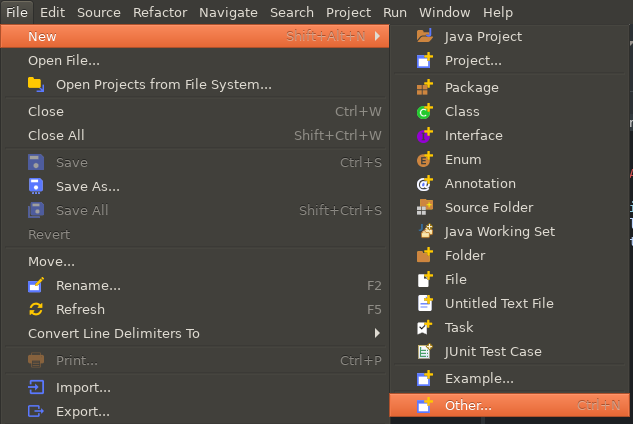
\includegraphics[width=0.9\linewidth, height=7cm]{3DependencyManagement/eclipsePlugin/newProject.png}
\end{subfigure}
\begin{subfigure}{0.5\textwidth}
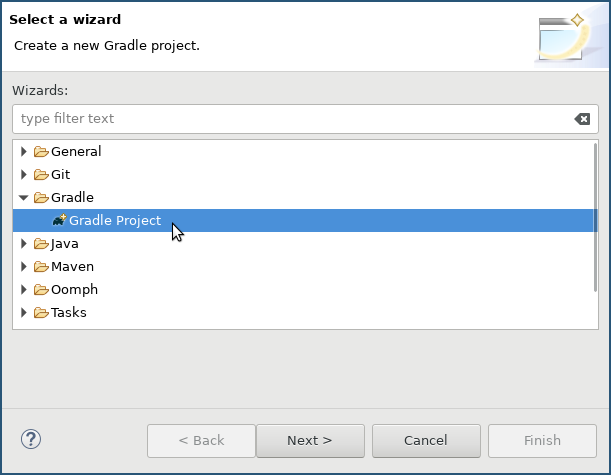
\includegraphics[width=0.9\linewidth, height=7cm]{3DependencyManagement/eclipsePlugin/wizardGradle.png}
\end{subfigure}
\end{figure}
Dopo aver indicato la posizione e il nome del progetto, sarà richiesto se usare il wrapper Gradle o di specificare la posizione in locale di Gradle. Ci sarà poi un riassunto generale e cliccando su finish il progetto verrà creato. Notiamo che non ci sono differenze tra la versione del progetto generata con questa modalità o con il procedimento da terminale, infatti eclipse automatizzerà solo i procedimenti di creazione ma non il modo di creazione. Il plugin di Gradle per eclipse mette a disposizione anche una versione grafica per eseguire le build includendo 2 finestre:
\begin{itemize}
    \item Gradle Tasks, che restituisce la lista dei tasks relativi al progetto selezionato
    \item Gradle Executions, che è in poche parole l'output della build eseguita in formato non terminale
\end{itemize}
Per poterle aggiungere dobbiamo andare su \texttt{Window -> Show View -> Other...} e poi selezionare le due view di Gradle:
\begin{figure}[H]
\begin{subfigure}{0.6\textwidth}
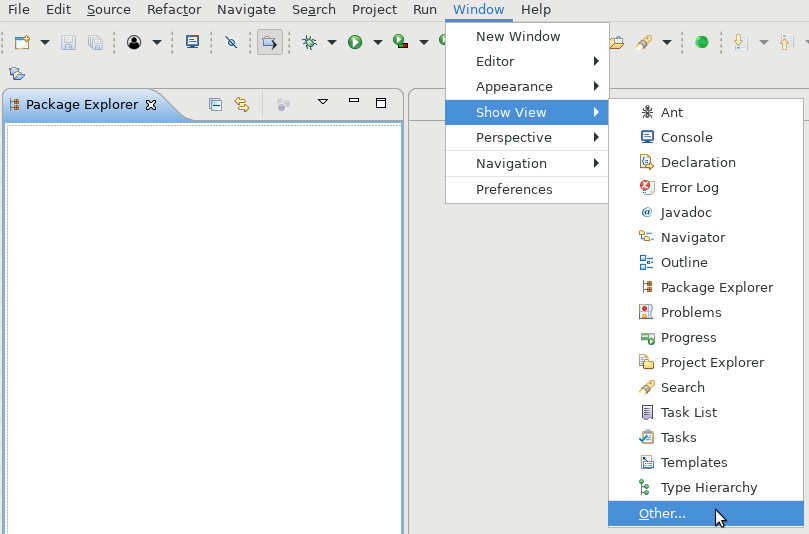
\includegraphics[width=1.0\linewidth, height=7cm]{3DependencyManagement/eclipsePlugin/openShowView.png}
\end{subfigure}
\begin{subfigure}{0.6\textwidth}
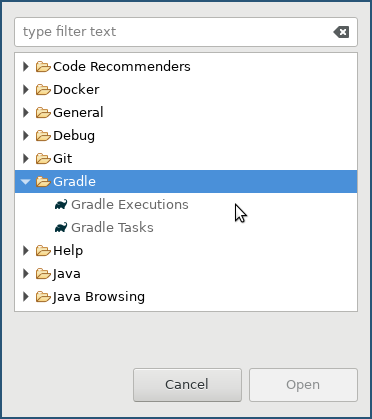
\includegraphics[width=0.6\linewidth, height=7cm]{3DependencyManagement/eclipsePlugin/gradlePluginFeature.png}
\end{subfigure}
\end{figure}
Usando questa view possiamo eseguire direttamente i task che vogliamo, per esempio se volessimo eseguire il task \texttt{test} basterà cliccare con il destro e poi su \texttt{Run Gradle Tasks}:
\begin{figure}[H]
    \centering
    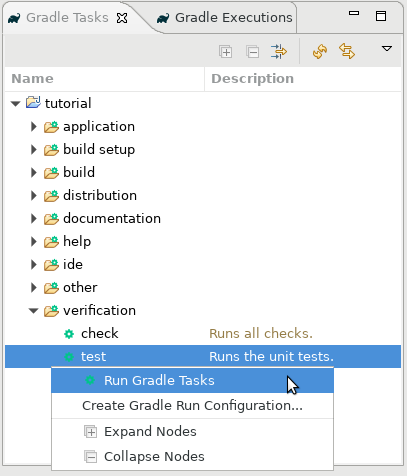
\includegraphics[width=0.4\linewidth]{3DependencyManagement/eclipsePlugin/runTestTask.png}
\end{figure}
Noteremo che sia la view  \texttt{Console} sia la view \texttt{Gradle Executions} si sono aggiornati, il primo con l'effettiva esecuzione del task mentre il secondo con una sorta di report:
\begin{figure}[H]
\begin{subfigure}{0.5\textwidth}
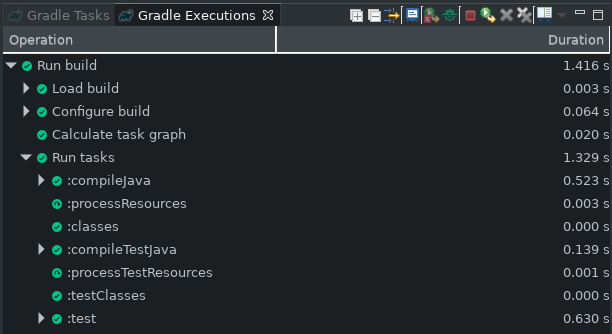
\includegraphics[width=1.0\linewidth, height=7cm]{3DependencyManagement/eclipsePlugin/gradleExecutionsView.png}
\end{subfigure}
\begin{subfigure}{0.5\textwidth}
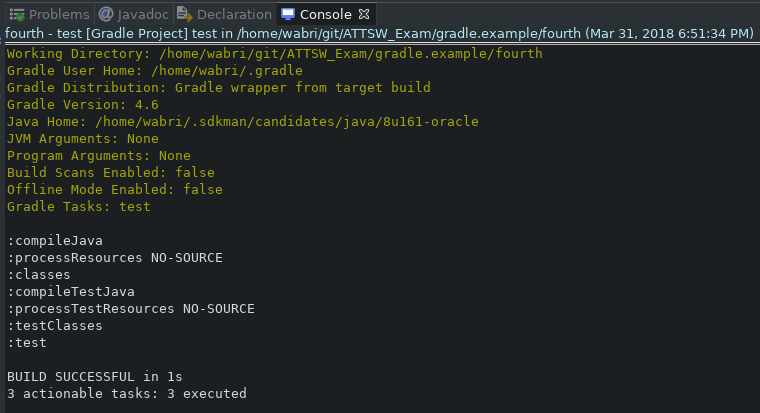
\includegraphics[width=1.1\linewidth, height=7cm]{3DependencyManagement/eclipsePlugin/consoleView.png}
\end{subfigure}
\end{figure}
Usando questi strumenti di Eclipse è possibile fare tutto ciò che prima veniva fatto da terminale.

\subsection{Tutorial}
Il tutorial di seguito è possibile anche trovarlo al link: \href{https://github.com/Wabri/ATTSW_Exam/blob/master/gradle.example/third/}{\textsc{github.com/Wabri/ATTSW\_Exam/blob/master/gradle.example/third/}}.
\begin{enumerate}
    \item Creare una cartella gradle.example/third
    \item Eseguire la build:
\begin{verbatim}
    $ gradle init --type java-application
\end{verbatim}
    \item Controllare e nel caso modificare il build.gradle per fare in modo di avere:
    \begin{itemize}
        \item il java plugin
        \item Come unica repository MavenCentral
        \item junit 4.12
    \end{itemize}
    \item Eseguire la build \texttt{dependencies} per scaricare le dipendenze
    \item Assicurarsi che junit sia configurato per il testImplementation, com'è possibile notare dal comando precedente la configurazione testCompile è deprecata
    \item Eseguire nuovamente la build \texttt{dependencies}, controllare se la dipendenza junit è stata associata alla configurazione testImplementation
    \item Eseguire la build di test con continuous:
    \begin{verbatim}
    $ ./gradlew test --continuous\end{verbatim}
    \item Aggiungere il metodo helloWorldSendTest nella classe di test AppTest:
    \begin{lstlisting}[frame=single]
    @Test 
    public void helloWorldSendTest () {
	    App classUnderTest = new App();
	    assertEquals("Hello world!", classUnderTest.getGreeting());
    }
    \end{lstlisting}
    Questo dovrà far fallire la build test avviata nel punto precedente.
    \item Correggere il test modificando il metodo getGreeting() nella classe App:
    \begin{lstlisting}[frame=single]
    public String getGreeting() {
        return "Hello world!";
    }
    \end{lstlisting}
    A questo punto la build test avrà successo.
    \item Stoppare la build test usando la combinazione \texttt{ctrl+d}
    \item Eseguire la build di test con continuous sul metodo testAppHasAGreeting():
    \begin{verbatim}
    $ ./gradlew test --continuous --tests AppTest.testAppHasAGreeting \end{verbatim}
    \item Modificare il metodo di test helloWorldSendTest:
    \begin{lstlisting}[frame=single]
    @Test 
    public void helloWorldSendTest () {
	    App classUnderTest = new App();
	    assertEquals("Greetings", classUnderTest.getGreeting());
    }
    \end{lstlisting}
    Ovviamente la build avrà successo dato che non stiamo modificando il metodo sotto test. Stoppare quindi la build usando \texttt{ctrl+d}
    \item Modificare il metodo getGreeting della classe App in modo da non far fallire la build:
    \begin{verbatim}
    $ ./gradlew test --continuous --tests \*Test\end{verbatim}
    \item Aggiungere il MANIFEST alla build.gradle:
    \begin{lstlisting}[frame=single]
    jar {
        manifest {
            attributes("Implementation-Title": "App","Implementation-Version":1.0,'Main-Class':'App')
        }
    }
    \end{lstlisting}
    \item Eseguire la build jar:
    \begin{verbatim}
        $ ./gradlew jar\end{verbatim}
    \item Provare ad eseguire l'applicativo appena creato (che si troverà nella directory build/libs/):
    \begin{verbatim}
        $ java -jar build/libs/third.jar \end{verbatim}
    Quello che dovrà comparire sarà la stringa di ritorno del metodo getGreeting().
    \item Aggiungere alla lista dei plugin quello di eclipse:
    \begin{lstlisting}[frame=single]
    id 'eclipse'
    \end{lstlisting}
    \item Eseguire la build di creazione metadati di eclipse:
    \begin{verbatim}
        $ ./gradlew eclipse \end{verbatim}
    \item Importare il progetto su eclipse:
    \begin{figure}[H]
        \begin{subfigure}{0.5\textwidth}
        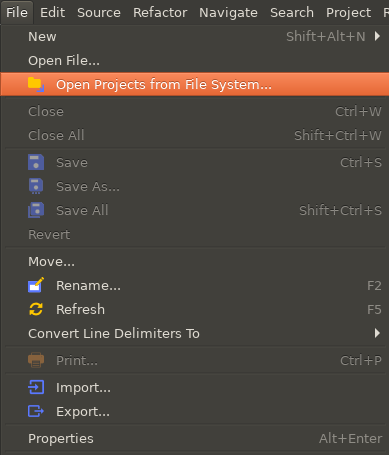
\includegraphics[width=1.0\linewidth, height=7cm]{3DependencyManagement/tutorial/importProject.png}
        \end{subfigure}
        \begin{subfigure}{0.5\textwidth}
        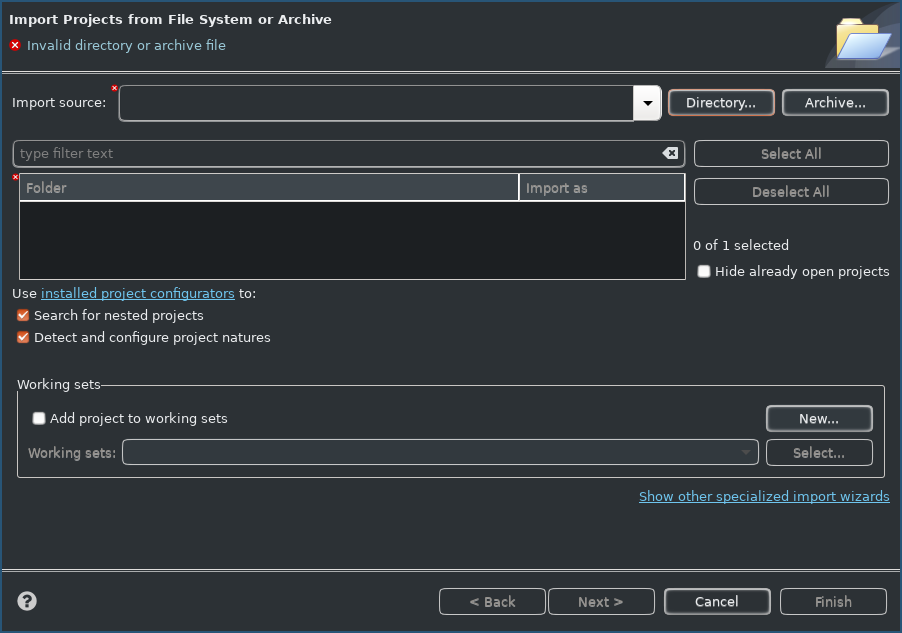
\includegraphics[width=1.0\linewidth, height=7cm]{3DependencyManagement/tutorial/importSource.png}
        \end{subfigure}
    \end{figure}
    \item Eseguire la build \texttt{test} usando la view \texttt{Gradle Tasks} di Eclipse
    \item Se la build di test è andata a buon fine allora eseguire la build \texttt{jar}, sempre usando il \texttt{Gradle Tasks}
    \item Testare il funzionamento dell'ultima build eseguendo da terminale il solito comando del punto 16
\end{enumerate}